\renewcommand{\arraystretch}{1.5}
\subsection{Grundelemente}
\begin{tabular}{p{1.5cm} p{4.3cm} |p{1.5cm} p{4.3cm}| p{1.5cm} p{4.3cm}}
	\multicolumn{2}{l}{\textbf{Ohmscher Widerstand R}}
	& \multicolumn{2}{l}{\textbf{Kapazitität C}}
	& \multicolumn{2}{l}{\textbf{Induktivität L}} \\
	\multicolumn{2}{l}{\textbf{u und i können sprunghaft ändern}}
	& \multicolumn{2}{l}{$\mathbf{u}$ \textbf{kann nicht sprunghaft ändern}}
	& \multicolumn{2}{l}{$\mathbf{i}$ \textbf{kann nicht sprunghaft ändern}} \\
	
	\multirow{2}{1.5cm}{
		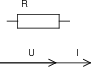
\includegraphics[width=1.5cm]{./images/zeigerdiag-r.png}}
	& $u(t) = R \cdot i(t)$ 
	& \multirow{2}{1.5cm}{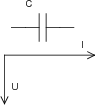
\includegraphics[width=1.5cm]{./images/zeigerdiag-c.png}}
	& $u(t) = \frac{1}{C} \int\limits_0^t i(\tau) d\tau + u(0)$
	& 
	\multirow{2}{1.5cm}{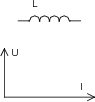
\includegraphics[width=1.5cm]{./images/zeigerdiag-l.png}}
	&$u(t) = L \frac{di(t)}{dt}$\\
	
	&$i(t) = \frac{u(t)}{R}$
	& & $i(t) = C \frac{d u(t)}{dt}$
	& & $i(t) = \frac{1}{L} \int\limits_0^t u(\tau) d\tau + i(0)$\\
	
	& $\underline{Z}_R = R$
	& & $\underline{Z}_C = \frac{1}{j \omega C} = - \frac{j}{\omega C}$
	& & $\underline{Z_L} = j \omega L$\\
	
	& 
	& & $X_C = -\frac{1}{\omega C} \quad B_C = \omega C$
	& & $X_L = \omega L
	\quad B_L = -\frac{1}{\omega L}$ \\
	
	& $P=I^2 \cdot R = \frac{U^2}{R}$
	& & $Q_C= - U^2 \cdot \omega C = - \frac{I^2}{\omega C}$
	& & $Q_L= I^2 \cdot \omega L = \frac{U^2}{\omega L}$\\
	
	& & & $W_C=\frac12 C U_C^2$
	& &$W_L=\frac12 L I_L^2$
\end{tabular}

%\subsection{Begriffe der Impedanz und Admittanz}
%\begin{tabular}{lllll}
%	Scheinwiderstand & & $Z = \frac{U_{eff}}{I_{eff}} $ & $ =
%	\sqrt{R^2+X^2}$ & Ohm\\ Komplexer Widerstand & Impedanz & $\underline Z = R + jX = Z \cdot e^{j \varphi}$ 
%	& $  = \dfrac{\underline{U}}{\underline{I}} = \dfrac{\underline{U}\cdot\underline{U}^{\ast}}{\underline{S}^*} =  \dfrac{U^2}{\underline{S}^*} = 
%	\dfrac{\underline{S}}{I^2}$ & Ohm\\
%	Komplexer Leitwert & Admittanz & $\underline Y = G + jB =
%	\frac{1}{\underline Z} = \frac{1}{Z}e^{-j\varphi}$ & $= \frac{\underline{I}}{\underline{U}}$ &  Siemens\\
%	Wirkwiderstand & Resistanz & $R = \Real(\underline Z) $ & $ = Z
%	\cdot cos(\varphi)$ & Ohm\\
%	Wirkleitwert & Konduktanz & $G = \Real(\underline Y) $ & $ \neq \frac{1}{R}$ &
%	Siemens\\
%	Blindwiderstand & Reaktanz & $X = \Imag(\underline Z) $ & $ = Z
%	\cdot sin(\varphi)$ & Ohm\\
%	Blindleitwert & Suszeptanz & $B = \Imag( \underline Y) $ & $ \neq \frac{1}{X}$
%	& Siemens\\
%	Phasenverschiebung & & $\varphi = \varphi_u - \varphi_i =
%	\arctan\left(\frac{\Imag(\underline{Z})}{\Real(\underline{Z})}\right)$ & &
%	Radiant\\	
%\end{tabular}
\clearpage